\documentclass[12pt]{article}

% --- Estilo base del usuario ---
\usepackage{setspace}
\usepackage{newtxtext,newtxmath}
\setstretch{1.5}

\usepackage{amsmath}
\usepackage[utf8]{inputenc}
\usepackage[spanish]{babel}
\usepackage[letterpaper, left=3cm, right=2.5cm, top=2.5cm, bottom=2.5cm]{geometry}

\usepackage{graphicx}
\usepackage{titlesec}
\usepackage{lipsum}
\usepackage{pdfpages}
\usepackage{comment}
\usepackage{float}
\usepackage{enumitem}
\graphicspath{{./Imagenes/}}

\usepackage{pdfpages}


\usepackage{siunitx}




%%%%%%%%% PAQUETES NUEVOS PARA SIMBOLOS%%%%%%%%%%%






\sisetup{
	output-decimal-marker = {,}, % imprime coma decimal
	group-separator       = {.}, % separador de miles
	group-minimum-digits  = 4,   % agrupar a partir de 4 dígitos (opcional)
	% opcional: aceptar tanto punto como coma en la entrada
	input-decimal-markers = {.,,}
}


%----Empezar cada section enuna hoja nueva 
\let\oldsection\section
\renewcommand{\section}{\clearpage\oldsection}


% --- Encabezado: número SOLO arriba derecha ---
\usepackage{fancyhdr}
\pagestyle{fancy}
\fancyhf{}
\fancyhead[R]{\thepage}
\renewcommand{\headrulewidth}{0pt}
\fancypagestyle{plain}{%
	\fancyhf{}
	\fancyhead[R]{\thepage}
	\renewcommand{\headrulewidth}{0pt}
}

% --- Tabla de contenido con líneas punteadas ---
\usepackage{tocloft}
\renewcommand{\cftsecleader}{\cftdotfill{\cftdotsep}}
\renewcommand{\cftdotsep}{1.5}
\renewcommand{\contentsname}{Contenido} % título del \tableofcontents


% --- Hipervínculos clicables en el índice (cargar casi al final) ---
\usepackage[hidelinks]{hyperref}
% Si prefieres verlos en color:
% \hypersetup{colorlinks=true, linkcolor=blue}
\usepackage{bookmark}
% Listas
\setlist[enumerate]{listparindent=\parindent, parsep=0pt}




\begin{document}
	
	% ===== ÍNDICE (no numera ni cuenta) =====
	\section*{Contenido} % título visible (no entra al TOC)
	\tableofcontents
	\thispagestyle{empty} % sin número en esta(s) página(s)
	\clearpage
	% Reiniciar para que "Objetivos" sea página 1
	\pagenumbering{arabic}
	\setcounter{page}{1}
	
	% ===== CONTENIDO =====
	\section{Objetivos}
	
	\subsection{Objetivo general}
	Fortalecer el proceso de enseñanza–aprendizaje durante mi práctica docente en el Laboratorio de Matemática Básica 1 mediante la planificación, impartición y evaluación de contenidos clave (ecuaciones lineales, geometría, funciones polinomiales, racionales, exponenciales–logarítmicas y trigonometría), incorporando recursos digitales (GeoGebra), seguimiento del desempeño estudiantil y cierre formativo con proyectos finales.
	
	\subsection{Objetivos específicos}
	\begin{itemize}
		\item Planificar y desarrollar sesiones de clase alineadas al programa, abarcando desde ecuaciones lineales y geometría básica hasta funciones polinomiales y sus aplicaciones.
		\item Implementar estrategias didácticas activas para la explicación, ejercitación guiada y resolución de problemas, promoviendo el razonamiento matemático del estudiantado.
		\item Integrar el uso de GeoGebra y otros recursos digitales para la representación y análisis de funciones (polinomiales, racionales, exponenciales y logarítmicas).
		\item Evaluar el aprendizaje mediante instrumentos formativos y sumativos (tareas, ejercicios y examen parcial), brindando retroalimentación oportuna y registrando avances.
		\item Coordinar y acompañar el cierre con proyectos finales, asegurando criterios claros de evaluación y evidencias del logro de los resultados de aprendizaje.
	\end{itemize}
	
	

	
	
	\section{Cronograma de actividades }
	\begin{figure}[H]
		\centering
		
\includegraphics[width=0.75\textwidth]{cronogramad}
		\caption{Cronograma de actividades de Práctica Docente.}
		\label{fig:losa2}
	\end{figure}
	

	
	\section{Introducción}
	
	La práctica docente se llevó a cabo en la ciudad de Quetzaltenango, en el Centro Universitario de Occidente (CUNOC) de la Universidad de San Carlos de Guatemala, dentro del curso Laboratorio de Matemática Básica 1, sección “B”. 
	
	El motivo de la colaboración surgió como parte del cumplimiento de las prácticas finales, brindando apoyo docente al Centro Universitario de Occidente. El propósito fue contribuir en la enseñanza del curso de Matemática Básica 1, orientando a los estudiantes de primer semestre en el desarrollo de los temas fundamentales del programa. 
	
	El objetivo principal fue aprovechar la experiencia adquirida como estudiantes que ya cursaron y aprobaron estas materias, para brindar una guía más cercana y comprensible a los alumnos. Asimismo, se buscó fortalecer habilidades personales como la comunicación oral, la confianza frente a grupos y la capacidad de liderazgo en el aula, fomentando un ambiente participativo y colaborativo.
	
	La metodología aplicada incluyó la planificación y ejecución de clases teóricas y prácticas, el uso de recursos tecnológicos como GeoGebra y la elaboración de hojas de trabajo orientadas al aprendizaje activo. Se desarrollaron ejercicios de aplicación, sesiones de resolución de problemas, supervisión de evaluaciones parciales y proyectos finales, abarcando temas como ecuaciones lineales, números complejos, geometría, funciones polinomiales, racionales, exponenciales, logarítmicas y trigonometría.
	
	Finalmente, los resultados obtenidos permitieron fortalecer las competencias docentes, mejorar la expresión oral y la gestión de grupo, además de adquirir experiencia práctica en el proceso de enseñanza universitaria. Entre las principales limitaciones se encontró el tiempo reducido para la atención individual de los estudiantes; sin embargo, la práctica resultó valiosa para consolidar tanto el aprendizaje profesional como el compromiso con la formación académica.
	
	
	
	
	%%%%%%%%%%%%%%%%%%%%%%%%%%%%%%%%%%%%%%%%%%%%%%%%%%%%
	%%%%%%%%%%%%%%% CAPITULO 1	
	
	\section{Capítulo 1}
	
	\subsection{Descripción del programa del curso}
	
	El Laboratorio de Matemática Básica 1 está orientado a aplicar y consolidar los contenidos del curso principal mediante trabajo práctico y guiado. Se desarrollan ejercicios y hojas de trabajo sobre ecuaciones lineales, números complejos, geometría básica, funciones polinomiales y racionales, así como exponenciales, logarítmicas y trigonometría; se utiliza GeoGebra para la representación y verificación de resultados. La metodología combina explicación breve, resolución de problemas, retroalimentación continua y evaluaciones parciales vinculadas a proyectos y actividades integradas. El enfoque busca fortalecer el razonamiento matemático, la interpretación gráfica, la comunicación de procedimientos y la autonomía del estudiante.
	
	
	
	\subsection{Temas que se abordaron en la práctica}
	
	Durante la práctica docente se desarrollaron diversos temas del programa oficial, siguiendo el orden del avance académico del curso. Entre los principales contenidos trabajados se incluyen:
	
	
	\begin{itemize}
		\item \textbf{Ecuaciones lineales y números complejos:} resolución de ecuaciones de primer grado y operaciones básicas con números complejos en forma binómica, con aplicaciones a problemas simples.
		\item \textbf{Geometría básica y resolución de ejercicios:} repaso de elementos, triángulos, polígonos y circunferencia; cálculo de longitudes, áreas y volúmenes en situaciones prácticas.
		\item \textbf{Análisis del primer examen parcial con GeoGebra:} retroalimentación de procedimientos y verificación gráfica/dinámica de resultados para consolidar criterios de solución.
		\item \textbf{Funciones polinomiales y su graficación:} identificación de grado, ceros y multiplicidad; construcción de tablas de valores y esbozo de la curva considerando comportamiento extremo.
		\item \textbf{Aplicaciones de funciones polinomiales:} modelado de fenómenos sencillos (costo–ingreso, trayectorias, ajustes por puntos) e interpretación de intervalos de positividad y extremos.
		\item \textbf{Funciones racionales:} análisis de dominio, intersecciones, asíntotas verticales/horizontales/oblicuas y discontinuidades, con lectura e interpretación de sus gráficas.
		\item \textbf{Funciones exponenciales y logarítmicas:} estudio de crecimiento/decaimiento, leyes de logaritmos, ecuaciones y modelos (interés compuesto, vida media, poblaciones).
		\item \textbf{Trigonometría (leyes de senos, cosenos y tangente):} resolución de triángulos, cálculo de alturas y distancias indirectas, rumbos y problemas de triangulación.
	\end{itemize}
	
	
	
	Cada tema fue abordado mediante clases expositivas, resolución de ejercicios, elaboración de hojas de trabajo, actividades de retroalimentación y orientación individual y grupal. Además, se colaboró en la aplicación de evaluaciones parciales, supervisión de proyectos finales y apoyo académico continuo a los estudiantes.
	
	\subsection{Habilidades desarrolladas}
	Durante la práctica docente se fortalecieron tanto competencias técnicas como pedagógicas. Entre las principales habilidades desarrolladas destacan:
	\begin{itemize}
		\item Capacidad para planificar, organizar e impartir clases siguiendo una secuencia lógica de contenidos.
		\item Mejora en la expresión oral, dominio del grupo y seguridad al hablar en público.
		\item Aplicación de recursos tecnológicos y didácticos (GeoGebra, presentaciones, hojas de trabajo) para facilitar la comprensión matemática.
		\item Evaluación y retroalimentación efectiva del aprendizaje de los estudiantes.
		\item Trabajo colaborativo con el docente titular y responsabilidad en la gestión académica.
	
	\end{itemize}
	En conjunto, estas habilidades contribuyeron al fortalecimiento del perfil profesional docente y a la comprensión del rol del educador como facilitador del aprendizaje activo y significativo.
	
	
	
	
	
	
	
	
	
	
	
	
	
	%%%%%%%%%%%%%%%%%%%%%%%%%%%%%%%%%%%%%%%%%%%%%%%%%%%%%	
	
	
		
	\section{Capítulo 2}
	
	
	\subsection{Ecuaciones lineales y números complejos}
	
	Las ecuaciones lineales son expresiones de primer grado que permiten relacionar una variable con una constante. Son la base del álgebra elemental y de numerosos modelos en ingeniería y ciencias aplicadas. Una ecuación lineal en una variable tiene la forma general:
	\[
	ax+b=0, \qquad a\neq0,
	\]
	y su solución se obtiene despejando:
	\[
	x=-\frac{b}{a}.
	\]
	En el caso de sistemas lineales de dos ecuaciones con dos incógnitas, se pueden resolver por métodos algebraicos como sustitución, igualación, eliminación o por la Regla de Cramer:
	\[
	\begin{cases}
		a_1x+b_1y=c_1,\\
		a_2x+b_2y=c_2,
	\end{cases}
	\quad
	x=\frac{\begin{vmatrix} c_1 & b_1 \\ c_2 & b_2 \end{vmatrix}}{\begin{vmatrix} a_1 & b_1 \\ a_2 & b_2 \end{vmatrix}},
	\qquad
	y=\frac{\begin{vmatrix} a_1 & c_1 \\ a_2 & c_2 \end{vmatrix}}{\begin{vmatrix} a_1 & b_1 \\ a_2 & b_2 \end{vmatrix}}.
	\]
	
	Por otro lado, los números complejos se representan como:
	\[
	z=a+bi,
	\]
	donde $a$ es la parte real, $b$ la parte imaginaria y $i$ la unidad imaginaria, definida por $i^2=-1$. Su forma polar es $z=r(\cos\theta+i\sin\theta)$, con $r=\sqrt{a^2+b^2}$.
	
	\textbf{Ejemplo:} Resolver $3x+6=0$ da como resultado $x=-2$. Para un número complejo $z=3+4i$, su módulo es $|z|=\sqrt{3^2+4^2}=5$ y su argumento $\theta=\tan^{-1}(4/3)\approx53.13^\circ$.
	
	\begin{figure}[H]
		\centering
		
\includegraphics[width=0.7\textwidth]{imagen1.jpg}
		\caption{Representación de ecuaciones lineales}
	\end{figure}
	
	
	\begin{figure}[H]
		\centering
		
\includegraphics[width=0.55\textwidth]{imagen1.1.jpg}
		\caption{números complejos en el plano.}
	\end{figure}
	
	
	
	---
	
	\subsection{Geometría básica y resolución de ejercicios}
	
	La geometría estudia las propiedades de las figuras y las relaciones métricas entre sus elementos. Es fundamental para comprender la estructura espacial, la medida y la forma de los cuerpos geométricos, tanto en el plano como en el espacio tridimensional.
	
	Algunas fórmulas básicas utilizadas en este curso son:
	\[
	A_{\triangle}=\frac{1}{2}bh, \qquad 
	A_{\text{círculo}}=\pi r^2, \qquad 
	L_{\text{circunferencia}}=2\pi r,
	\]
	\[
	A_{\text{rectángulo}}=b\cdot h, \qquad
	A_{\text{cuadrado}}=l^2, \qquad
	A_{\text{trapecio}}=\frac{(B+b)h}{2}.
	\]
	
	\begin{figure}[H]
		\centering
		
\includegraphics[width=0.7\textwidth]{imagen2.1.jpg}
		\caption{Formulas de Geometría .}
	\end{figure}
	
		
	\begin{figure}[H]
		\centering
		
\includegraphics[width=0.7\textwidth]{imagen2.jpg}
		\caption{Elementos de Geometría}
	\end{figure}
	
	El teorema de Pitágoras se aplica a triángulos rectángulos:
	\[
	a^2+b^2=c^2.
	\]
	
	\begin{figure}[H]
		\centering
		
\includegraphics[width=0.7\textwidth]{imagen2.3.jpg}
		\caption{Representación de Formula Cuadrática }
	\end{figure}

	
	\textbf{Ejemplo:} En un triángulo con base $b=8$ cm y altura $h=5$ cm, su área es:
	\[
	A=\frac{1}{2}(8)(5)=20\ \text{cm}^2.
	\]
	Si el triángulo es rectángulo con catetos de 6 y 8 cm, la hipotenusa será $c=\sqrt{6^2+8^2}=10$ cm.

	

	
	\subsection{Funciones polinomiales y su graficación}
	
	Una función polinomial está compuesta por la suma de potencias de una variable multiplicadas por coeficientes constantes:
	\[
	f(x)=a_nx^n+a_{n-1}x^{n-1}+\dots+a_1x+a_0.
	\]
	Estas funciones son continuas y derivables en todo $\mathbb{R}$, y su forma gráfica depende del grado $n$ y del signo del coeficiente principal $a_n$.  
	Las raíces del polinomio determinan los puntos donde la función corta el eje $x$.
	
	\begin{figure}[H]
		\centering
		
\includegraphics[width=0.55\textwidth]{imagen3.jpg}
		\caption{Representacion funciones polinomiales.}
	\end{figure}
	
	Para el caso de una función cuadrática ($n=2$):
	\[
	f(x)=ax^2+bx+c,
	\]
	su vértice se calcula como:
	\[
	x_v=-\frac{b}{2a}, \qquad y_v=f(x_v),
	\]
	y su eje de simetría corresponde a la recta $x=x_v$.
	
	\textbf{Ejemplo:} Dada la función $f(x)=x^2-4x+3$, el vértice es $(2,-1)$, las raíces son $x=1$ y $x=3$, y la parábola abre hacia arriba.
	

	
	
		\begin{figure}[H]
		\centering
		
\includegraphics[width=0.55\textwidth]{imagen3.1.jpg}
		\caption{Gráfica de Polinomios }
	\end{figure}
	
	---
	
	\subsection{Aplicaciones de funciones polinomiales}
	
	Las funciones polinomiales se aplican para representar fenómenos de la vida real como trayectorias, crecimiento, costos o ingresos. Un caso frecuente es el de la función de utilidad:
	\[
	U(x)=I(x)-C(x),
	\]
	donde $I(x)$ representa el ingreso y $C(x)$ el costo.
	
	\textbf{Ejemplo:} Si $I(x)=50x$ y $C(x)=2x^2+20x$, entonces:
	\[
	U(x)=50x-(2x^2+20x)=-2x^2+30x.
	\]
	El punto de máxima utilidad se determina derivando:
	\[
	U'(x)=-4x+30=0\Rightarrow x=7.5,
	\]
	por lo tanto, la máxima utilidad se obtiene cuando se producen $7.5$ unidades.
	
	\begin{figure}[H]
		\centering
		
\includegraphics[width=0.55\textwidth]{imagen4.jpg}
		\caption{Modelo económico representado mediante una función polinomial.}
	\end{figure}
	
	---
	
	\subsection{Funciones racionales: dominio, asíntotas e intersecciones}
	
	Una función racional es aquella que se expresa como el cociente de dos polinomios:
	\[
	f(x)=\frac{p(x)}{q(x)}, \quad q(x)\neq0.
	\]
	Su dominio son todos los valores reales para los cuales $q(x)\neq0$.  
	Presenta asíntotas verticales cuando el denominador se anula y horizontales u oblicuas dependiendo de los grados de $p(x)$ y $q(x)$:
	\[
	\text{Si } \deg(p)<\deg(q), \text{ entonces } y=0;
	\quad
	\text{si } \deg(p)=\deg(q), \text{ entonces } y=\frac{a_n}{b_m}.
	\]
	
	\begin{figure}[H]
		\centering
		
\includegraphics[height=8cm,keepaspectratio]{imagen5}\hfill
		
\includegraphics[height=8cm,keepaspectratio]{imagen5.1}
		\caption{Comportamiento gráfico de una función racional con discontinuidad}
	\end{figure}
	
	\textbf{Ejemplo:} Para $f(x)=\dfrac{x^2-1}{x-1}$, al simplificar se obtiene $f(x)=x+1$ con una discontinuidad en $x=1$.  
	El dominio es $\mathbb{R}\setminus\{1\}$, sin asíntota vertical y sin asíntota horizontal.
	
		\begin{figure}[H]
		\centering
		
\includegraphics[height=7cm,keepaspectratio]{imagen5.2}\hfill
		
\includegraphics[height=7cm,keepaspectratio]{imagen5.3}
		\caption{Comportamiento gráfico de una función racional con discontinuidad}
	\end{figure}
	

	
	\subsection{Funciones exponenciales y logarítmicas}
	
	Las funciones exponenciales y logarítmicas permiten modelar procesos de crecimiento y decrecimiento continuo.  
	Una función exponencial tiene la forma:
	
	\begin{figure}[H]
		\centering
		
\includegraphics[width=0.3\textwidth]{imagen6.jpg}
		\caption{Gráficas de funciones exponenciales y logarítmicas.}
	\end{figure}
	
	
	\[
	f(x)=a^x, \quad a>0, a\neq1,
	\]
	mientras que su inversa, la función logarítmica, se expresa como:
	\[
	g(x)=\log_a x.
	\]
	Estas funciones son fundamentales en el estudio de fenómenos naturales, financieros y poblacionales.
	
		\begin{figure}[H]
		\centering
		
\includegraphics[height=8cm,keepaspectratio]{imagen6.1}\hfill
		
\includegraphics[height=8cm,keepaspectratio]{imagen6.2}
		\caption{Gráficas de funciones exponenciales y logarítmicas}
	\end{figure}
	
	\textbf{Ejemplo:} En un modelo de crecimiento poblacional:
	\[
	P(t)=P_0e^{kt},
	\]
	si $P_0=500$ y $k=0.04$, después de 5 años:
	\[
	P(5)=500e^{0.2}\approx610.7.
	\]
	
	\begin{figure}[H]
		\centering
		
\includegraphics[width=0.8\textwidth]{imagen6.3.jpg}
		\caption{Gráficas de un modelo Exponencial}
	\end{figure}
	
	
	
	\subsection{Trigonometría: leyes de senos, cosenos y tangente}
	
	La trigonometría relaciona los lados y ángulos de los triángulos, siendo de gran utilidad en problemas de medición, navegación y topografía.  
	Las principales relaciones trigonométricas son:
	
	\[
	\frac{a}{\sin A}=\frac{b}{\sin B}=\frac{c}{\sin C} \quad \text{(Ley de Senos)},
	\]
	
	\begin{figure}[H]
		\centering
		
\includegraphics[width=0.8\textwidth]{imagen7.jpg}
		\caption{Aplicación de las leyes trigonométricas para resolución de triángulos.}
	\end{figure}
	
	
	\[
	a^2=b^2+c^2-2bc\cos A \quad \text{(Ley de Cosenos)},
	\]
	
		\begin{figure}[H]
		\centering
		
\includegraphics[width=0.8\textwidth]{imagen7.1.jpg}
		\caption{Aplicación de las leyes trigonométricas para resolución de triángulos.}
	\end{figure}
	
	\[
	\frac{a-b}{a+b}=\frac{\tan\left(\tfrac{A-B}{2}\right)}{\tan\left(\tfrac{A+B}{2}\right)} \quad \text{(Ley de la Tangente)}.
	\]
	
			\begin{figure}[H]
		\centering
		
\includegraphics[width=0.8\textwidth]{imagen7.2.jpg}
		\caption{Aplicación de las leyes trigonométricas para resolución de triángulos.}
	\end{figure}
	
	\textbf{Ejemplo:} Para un triángulo con $b=8$, $c=6$ y $A=60^\circ$:
	\[
	a^2=8^2+6^2-2(8)(6)\cos60^\circ=100-48=52,
	\quad a\approx7.21.
	\]
	

	
	
	
	
	
	
	
	
	
	
	
	

	
	
	
	
	
	
	%%%%%%%%%%%%%%%%%%%%%%%%%%%hasa acaaaaaaaaaaaaaaaaaa
	
	
	
	
	
	
	
	






	
	
	\section{Capítulo 3}
	% ===========================
	% DESARROLLO DE FOLIOS
	% ===========================
	

\subsection{Folio 1}
\textbf{Clase impartida y Resolución de ejercicios}

Se realizo una breve presentación sobre la metodología de la clase, y se impartieron los temas de ecuaciones lineales y tomando en cuenta algunos temas sobre geometría, los contenidos que se abordaron fueron como un repaso de forma general debido a que el inicio de laboratorio no empezó en la fecha programada curso.

\begin{figure}[H]\centering
	
\includegraphics[width=0.85\textwidth]{fol2.jpg}
	\caption{Estudiantes Laboratorio Matemática Básicad 1}
\end{figure}


En cuanto a las ecuaciones se explicaron conceptos y métodos de resolución, verificando los resultados que se explicaron y los procedimientos. Con respecto a los números complejos, se trabajó la forma binómica y la representación en un plano complejo y operaciones básicas, aplicándolas a las ecuaciones que no tienen solución real


\begin{figure}[H]\centering
	
\includegraphics[width=1\textwidth]{fol4.jpg}
	\caption{Primer hoja de trabajo}
\end{figure}

Como se mencionó previamente debido a que el laboratorio no empezó en la fecha estipulada, por lo que se explicaron elementos básicos de geometría, Asimismo, durante la semana se revisaron tareas y hojas de trabajo, verificando procedimientos y resultados. Se realizó una investigación conceptual que incluyó un resumen teórico, la selección de ejemplos y otros insumos para fortalecer la preparación de clase. Finalmente, se elaboraron hojas de trabajo orientadas al aprendizaje activo.



\subsection{Folio 2}
\textbf{Clase impartida y asignación de hoja de trabajo:}

Previamente a la asignación de la actividad, se impartió un breve repaso sobre geometría, el contenido fue sobre las áreas de figuras planas y volumen de sólidos, con un enfoque en la compresión y deducción de las fórmulas y sus relaciones geométricas. Adicionalmente, se introdujo brevemente en el tema de funciones, revisando conceptos y representaciones elementales.

\begin{figure}[H]\centering
	
\includegraphics[width=0.3\textwidth]{fol5.jpg}
	\caption{Clase impartida sobre áreas y figuras geométricas.}
\end{figure}

Así también durante los días de clase se resolvieron dudas sobre los temas vistos, previo a la primera evaluación al cual los estudiantes se iban a someter al curso principal. Por consiguiente, se brindo apoyó al ingeniero Erick Coti titular de curso, en la supervisión de la evaluación escrita. Así mismo, se colaboró en la verificación de asistencia y el cumplimiento de las normas durante la prueba.




\begin{figure}[H]\centering
	
\includegraphics[width=0.6\textwidth]{fol6.jpg}
	\caption{Resolución de Ejemplo}
\end{figure}


Asimismo, durante la semana se revisaron tareas y hojas de trabajo, verificando procedimientos y resultados. Se realizó una investigación conceptual que incluyó un resumen teórico, la selección de ejemplos y otros insumos para fortalecer la preparación de clase. Finalmente, se elaboraron hojas de trabajo orientadas al aprendizaje activo.



\begin{figure}[H]\centering
	
\includegraphics[width=0.6\textwidth]{fol7.jpg}
	\caption{Resolución de Ejemplo.}
\end{figure}


\subsection{Folio 3}
\textbf{Resolución de Primer Examen Parcial}

Se analizo y se resolvió el primer examen parcial, aclarando dudas y explicando los procedimientos correctos a manera de retroalimentación, lo que permitió a los alumnos reconocer sus errores e identificar las áreas donde tienen que mejorar.

\begin{figure}[H]\centering
	
\includegraphics[width=0.85\textwidth]{fol8.jpg}
	\caption{Retroalimentación del primer parcial; funciones, plano coordenado, dominio y rango, con verificación gráfica en GeoGebra y revisión de tareas.}
\end{figure}

Así también se enfatizó y amplio el concepto de funciones, se definió lo que es el plano coordenado, traficación de ecuaciones, así mismo se establecieron nociones sobre dominio y rango. Se graficaron algunas funciones de manera que se combinó la explicación teórica con la introducción al software llamado GeoGebra, que es un software gratuito de graficación matemática 2D/3D que también permite trazar y analizar funciones y ecuaciones.

Asimismo, durante la semana se revisaron tareas y hojas de trabajo, verificando procedimientos y resultados. Se realizó una investigación conceptual que incluyó un resumen teórico, la selección de ejemplos y otros insumos para fortalecer la preparación de clase. Finalmente, se elaboraron hojas de trabajo orientadas al aprendizaje activo.

\begin{figure}[H]\centering
	
\includegraphics[width=0.7\textwidth]{fol9.jpg}
	\caption{Ejemplos sobre graficas de funciones}
\end{figure}


\subsection{Folio 4}
\textbf{Clase impartida e investigación teorica}

Se asigno una previa investigación conceptual acerca del tema que se tenía asignado el cual fue funciones polinomiales, esta actividad fue para que se relacionaran con el contenido y tuvieran una base teórica previa.

\begin{figure}[H]\centering
	
\includegraphics[width=0.3\textwidth]{fol10.jpg}
	\caption{Clase impartida a Estudiantes de Lab MB1.}
\end{figure}

Media vez se tuvo una introducción conceptual, se abordo la metodología de graficación de funciones polinomiales, detallando métodos como: tabla de valores, factorización para ceros, multiplicidad y extremos relativos. Para aplicar estos métodos se asignó una hoja de trabajo, en el cual se consideró la dinámica en que las gráficas fueran en el software de GeoGebra

\begin{figure}[H]\centering
	
\includegraphics[width=0.6\textwidth]{fol11.jpg}
	\caption{Investigación Teórica.}
\end{figure}

Asimismo, durante la semana se revisaron tareas y hojas de trabajo, verificando procedimientos y resultados. Se realizó una investigación conceptual que incluyó un resumen teórico, la selección de ejemplos y otros insumos para fortalecer la preparación de clase. Finalmente, se elaboraron hojas de trabajo orientadas al aprendizaje activo.




\subsection{Folio 5}
\textbf{Clase impartida: funciones polinomiales y su representación}

Se trabajó la estructura y análisis de polinomios (grado, término líder, ceros y multiplicidad) y su relación con la gráfica. Se factorizaron expresiones para hallar ceros e intersecciones con los ejes; luego se construyeron tablas de valores y se bosquejó la representación gráfica considerando comportamiento extremo y cambios cualitativos. Se usó GeoGebra para corroborar resultados y discutir la influencia de coeficientes en la forma de la curva.

\begin{figure}[H]\centering
	
\includegraphics[width=0.7\textwidth]{fol5.1.jpg}
	\caption{Serie de problemas de polinomios.}
\end{figure}

Como aplicaciones, se modelaron situaciones sencillas (costo–ingreso, trayectoria unidimensional, ajuste por ceros dados) interpretando intervalos de positividad y extremos. Se revisaron hojas de trabajo y se dio retroalimentación breve.



\begin{figure}[H]\centering
	
\includegraphics[width=0.85\textwidth]{fol5.2.jpg}
	\caption{Division larga de Polinomios}
\end{figure}
\subsection{Folio 6}
\textbf{Semana de asueto y revisión de material académico}

Durante esta semana no se impartieron clases presenciales debido al feriado del 15 de septiembre, conmemoración de la Independencia de Guatemala. No obstante, se aprovechó el tiempo para revisar hojas de trabajo y dar seguimiento académico a los estudiantes en los temas de funciones polinomiales



\subsection{Folio 7}
\textbf{Apoyo en la aplicación del Segundo Examen Parcial y profundización en aplicaciones de polinomios}

Durante la semana se colaboró con el ingeniero titular en la aplicación y supervisión del segundo examen parcial, apoyando en organización de aula, control de asistencia y cumplimiento de normas. Paralelamente, se profundizó en las aplicaciones de las funciones polinomiales, desarrollando casos de modelado (costos/ingresos, trayectorias y ajuste por ceros/puntos dados), interpretación de intervalos de positividad/negatividad y análisis de máximos y mínimos locales vinculados al contexto.

\begin{figure}[H]\centering
	
\includegraphics[width=0.85\textwidth]{fol7.1.jpg}
	\caption{Apoyo operativo al segundo parcial }
\end{figure}

\begin{figure}[H]\centering
	
\includegraphics[width=0.4\textwidth]{imagen4.jpg}
	\caption{ modelado, intervalos, máximos y mínimos.}
\end{figure}




\subsection{Folio 8}
\textbf{Clase impartida e investigación teorica sobre funciones racionales.}

Esta semana, por el Congreso CLEIMI, no hubo actividades con ponderación. Aun así, se avanzó en funciones racionales: dominio (restricciones del denominador), intersecciones, asíntotas verticales y horizontales/oblicuas, y discontinuidades. Se revisaron aplicaciones (tasas, costos promedio, mezclas) y la lectura modelo, gráfica e interpretación con verificación rápida en GeoGebra.

\begin{figure}[H]\centering
	
\includegraphics[width=0.99\textwidth]{fol8.1.jpg}
	\caption{Función Racional y su representación}
\end{figure}


\begin{figure}[H]\centering
	
\includegraphics[width=0.99\textwidth]{fol8.2.jpg}
	\caption{Resolución de Funciones Racionales}
\end{figure}

\subsection{Folio 9}
\textbf{Organización de grupos y avance en funciones racionales}

Durante la semana se organizaron grupos de trabajo para el proyecto final, estableciendo como fecha de entrega el 23 de octubre. Se explicó la estructura y criterios de evaluación del proyecto, así como los objetivos de aplicación práctica de los contenidos del curso.

\begin{figure}[H]\centering
	
\includegraphics[width=0.85\textwidth]{fol9.2.jpg}
	\caption{Organización de grupos para Proyecto Final.}
\end{figure}

Además, se impartió clase para ampliar el tema de funciones racionales, reforzando el análisis de dominio, intersecciones, asíntotas y discontinuidades. Como complemento, se asignó una hoja de trabajo enfocada en ejercicios de interpretación y aplicación de este tipo de funciones, promoviendo la consolidación del aprendizaje previo y su uso en contextos reales.

\begin{figure}[H]\centering
	
\includegraphics[width=0.85\textwidth]{fol9.1.jpg}
	\caption{Grafiando Funciones Racionales e identificación de Puntos.}
\end{figure}

\begin{figure}[H]\centering
	
\includegraphics[width=0.85\textwidth]{fol9.3.jpg}
	\caption{Graficando Asíntotas, horizontales, verticales y oblicuas}
\end{figure}


\subsection{Folio 10}
\textbf{Análisis y aplicaciones de funciones exponenciales y logarítmicas}

Esta semana se impartió funciones exponenciales y logarítmicas, enfatizando dominio y rango, asíntotas, transformaciones, crecimiento y decaimiento, y la relación de inversión entre ambas familias. En aplicaciones se trabajó: tasas de crecimiento y disminución, interés compuesto y continuo, vida media y desintegración, modelación de poblaciones, procesos físicos y escenarios financieros.
\begin{figure}[H]\centering
	
\includegraphics[width=0.50\textwidth]{fol10.1.jpg}
	\caption{Estudiantes de Laboratorio de Matemática Basica 1, Sección B}
\end{figure}

Como cierre, se asignó una hoja de trabajo para consolidar resolución de ejercicios, análisis de gráficos y planteamiento de modelos en contextos reales.

\begin{figure}[H]\centering
	
\includegraphics[width=0.70\textwidth]{fol10.2.jpg}
	\caption{Resolución de ejemplo en clase sobre Funciones exponenciales}
\end{figure}

\begin{figure}[H]\centering
	
\includegraphics[width=0.85\textwidth]{fol10.3.jpg}
	\caption{Resolución de problema con aplicación logarítmica }
\end{figure}




\subsection{Folio 11}
\textbf{Clase impartida sobre trigonometría (ley de senos, cosenos y tangente) y cierre de proyectos finales}

Esta semana se trabajó resolución de triángulos mediante ley de senos, cosenos y tangente, enfatizando criterios de selección del método según los datos disponibles, análisis de casos ambiguos, lectura e interpretación de diagramas y validación de resultados con estimaciones geométricas. Se abordaron aplicaciones en cálculo de alturas, distancias indirectas, rumbos y problemas de triangulación. Asimismo, se recibieron los proyectos finales por grupos, se revisó su cumplimiento de objetivos, coherencia metodológica y calidad de la presentación técnica; se brindó retroalimentación puntual y se realizó la actualización de notas y registros correspondientes en el control académico.

\begin{figure}[H]\centering
	
\includegraphics[width=0.85\textwidth]{fol11.1.jpg}
	\caption{Trigonometría aplicada: leyes de senos, cosenos y tangente; resolución de triángulos.}
\end{figure}
	
	\begin{figure}[H]\centering
		
\includegraphics[width=0.60\textwidth]{fol11.2.jpg}
		\caption{Resolución de Aplicación de Trigonometría.}
	\end{figure}
	
	
	
		\begin{figure}[H]\centering
		
\includegraphics[width=.99\textwidth]{fol11.3.jpg}
		\caption{Resolución de Aplicación de Trigonometría}
	\end{figure}
	
	
	
	
	
	
	
	
	
	
	
	
	
	
	
	
	
	%%%%%%%%%%%%%%%%%%%%%%%%%%%%%%%%%%%%%%%%%%%%%%%%%%%%%%%%%%%%%%%%%%%%%
	
	\section{Capitulo 4}
	
	\subsection{Actividades realizadas con enfoque GIRD y ACC }
	
	Durante el proceso de la práctica docente en el Laboratorio de Matemática Básica 1, sección B, se promovió la participaron activamente en actividades extracurriculares vinculadas al GIRD (Gestión Integral del Riesgo de Desastres) y al ACC
	
	Una de las principales actividades desarrolladas fue la \textbf{jornada de reforestación de árboles}, en la cual los estudiantes colaboraron en la siembra de especies nativas en áreas verdes en el municipio de cantel por el área de la granja penal. Esta acción tuvo como propósito fortalecer la conciencia ambiental, contribuir a la mitigación del cambio climático y fomentar el compromiso social de la comunidad estudiantil con el entorno natural. En este contexto, los principios de ACC se aplicaron al promover prácticas sostenibles que ayudan a restaurar ecosistemas locales y a reducir los efectos de la deforestación, vinculando así la educación con la acción ambiental responsable.
	
		\begin{figure}[H]\centering
		
\includegraphics[width=0.50\textwidth]{gird.jpg}
		\caption{Estudiantes de Laboratorio de Matemática Basica 1, participando en jornada de reforestación }
	\end{figure}
	
	Asimismo, los estudiantes también participaron en la Carrera 6K CUNOC, una actividad deportiva que tuvo su punto de partida en el Centro Universitario de Occidente y que buscó integrara los estudiantes de laboratorio de matemática básica 1, en acciones de convivencia saludable, promoción del bienestar físico y sensibilización sobre la importancia del espacio público seguro y sostenible. Desde el enfoque de GIRD, esta actividad fortaleció el sentido de organización, la prevención de riesgos en eventos masivos y la responsabilidad colectiva en el uso ordenado del entorno.
	

	
	\begin{figure}[H]\centering
		
\includegraphics[width=0.50\textwidth]{acc.jpg}
		\caption{Estudiantes de Laboratorio de Matemática Basica 1, participando en carrera }
	\end{figure}
	


	
	
	
	
	
	
	
	
	
	
	

	
	
	%%%%%%%%%%%%%%%%%%%%%%%%%%%%%%%%%%%%%%
	
	\section{Conclusiones}
	
	\subsection{Conclusiones}
	
	La práctica docente en el Laboratorio de Matemática Básica 1 permitió cumplir los objetivos propuestos al integrar una planificación clara, el uso sistemático de materiales de apoyo y la aplicación de estrategias didácticas activas. A lo largo del proceso se abordaron contenidos clave —ecuaciones lineales, geometría básica, funciones polinomiales y racionales, exponenciales y logarítmicas, y trigonometría— reforzando el vínculo entre teoría y práctica mediante hojas de trabajo, resolución guiada de ejercicios y la verificación con recursos digitales como GeoGebra. Esta combinación favoreció la comprensión conceptual y el razonamiento matemático, además de asegurar un avance ordenado y progresivo en el programa.
	
	La evaluación continua, basada en tareas, ejercicios aplicados y pruebas parciales, ofreció evidencia del aprendizaje y facilitó la retroalimentación oportuna. Se identificaron dificultades recurrentes —especialmente en la interpretación de gráficas y en la modelación básica— que fueron atendidas con ajustes metodológicos y apoyos específicos. El resultado fue un incremento en la autonomía del estudiante para seleccionar procedimientos, justificar pasos y validar resultados, fortaleciendo además la comunicación matemática y la lectura crítica de modelos en contextos reales.
	
	En el plano formativo y profesional, la práctica consolidó habilidades docentes como la organización del grupo, la comunicación efectiva y el liderazgo pedagógico, al tiempo que promovió una actitud reflexiva para adaptar estrategias a las necesidades del aula. Asimismo, la participación estudiantil en actividades con enfoque GIRD y ACC (reforestación y carrera 6K) integró principios de sostenibilidad y gestión del riesgo al quehacer académico, reforzando el compromiso social y ambiental. En conjunto, la experiencia evidenció que la articulación entre planificación, evaluación formativa y uso de tecnología potencia un aprendizaje significativo y pertinente para la formación en ingeniería.
	
	
	
	
	
	

	
	\section{Recomendaciones}
	
	\subsection{Recomendaciones (síntesis)}
	Para optimizar la práctica docente en el Laboratorio de Matemática Básica 1, se recomienda planificar cada clase con aplicaciones apegadas a la realidad para que el aprendizaje sea mas ágil y el estudiantado retengan mas información 
	
	Así también utilizar metodologías activas combinando la tecnología como  GeoGebra y otros software de graficación  de esa manera fortalecer la interpretación gráfica; Por consiguiente aplicar evaluación formativa mediante hojas de trabajo y ejercicios resueltos en clase.
	
	Fomentar la participación del los estudiantes con problemas matemáticos vinculados con problemas sociales para tener un mayor razonamiento matemático.
	
	Para tareas mas generales y extensas formar grupos en función de la cantidad de alumnos, ya que eso agiliza la calificación y por lo tanto las ponderaciones se proporcionan en un tiempo oportuno.
	
	
	
	\subsection{Bibliografía }
	
	\begin{enumerate}
		\item Stewart, J., Redlin, L., \& Watson, S. (s. f.). \textit{Precálculo: Matemáticas para el cálculo} (7.\textsuperscript{a} ed.). Cengage Learning.
		
		\item Swokowski, E. W., \& Cole, J. A. (s. f.). \textit{Álgebra y trigonometría con geometría analítica} (13.\textsuperscript{a} ed.). Cengage Learning.
		
		\item Zill, D. G., \& Dewar, J. M. (s. f.). \textit{Álgebra, trigonometría y geometría analítica}. Cengage Learning.
		
		\item Castillo, M. (s. f.). \textit{Geometría}. Departamento de Matemática, Universidad de San Carlos de Guatemala.
		
		\item Universidad de San Carlos de Guatemala. (s. f.). \textit{1.1 Ecuaciones}. Recursos de Matemática en Línea. Recuperado de \url{https://matematicaenlinea.com/basica-1/unidad-1-ecuaciones-y-desigualdades/1-1-ecuaciones/}
		
		\item Universidad de San Carlos de Guatemala, Centro Universitario de Occidente (CUNOC). (2025). \textit{Programa de curso: Área Matemática Básica 1} [Documento institucional].
	\end{enumerate}
	
	% Nota: Se usó (s. f.) cuando no se contó con el año exacto de publicación de la edición consultada.
	
	
		
	\subsection{Anexos}
	
	
	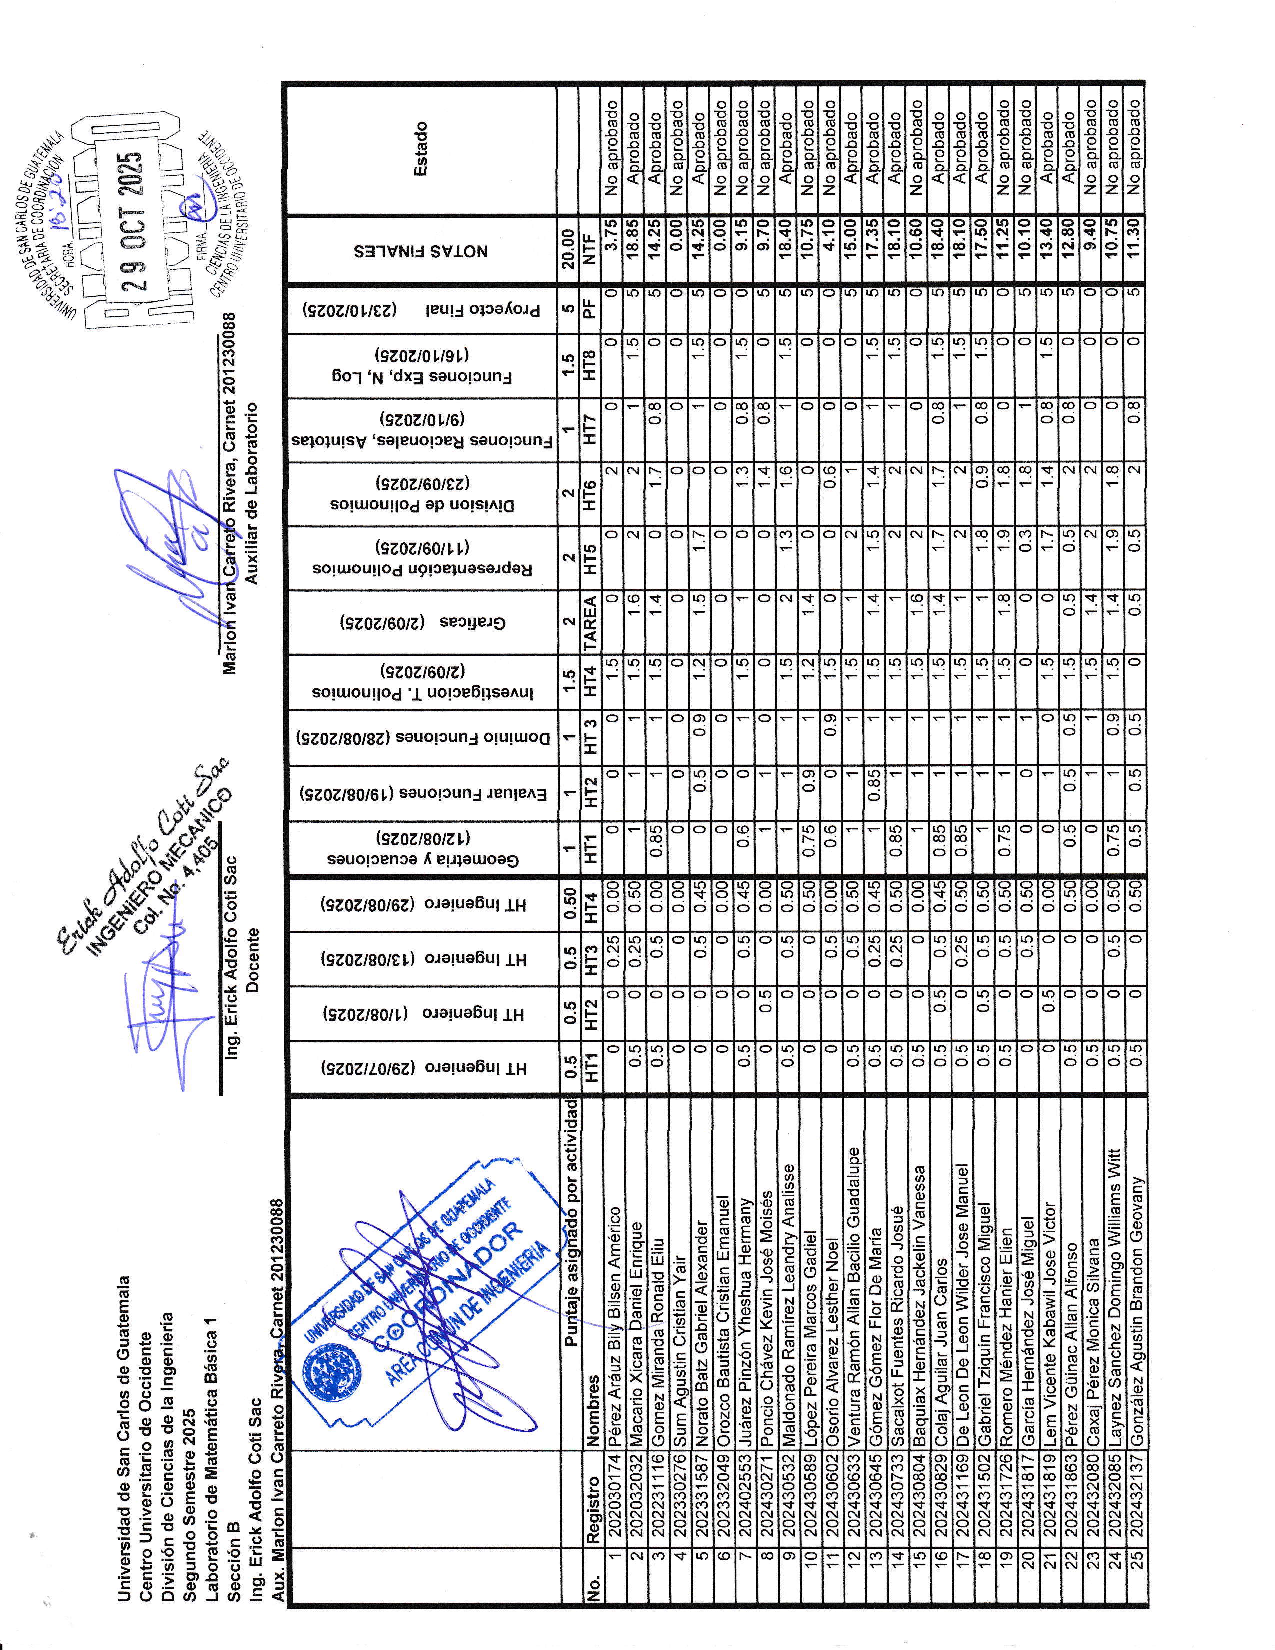
\includepdf[
	pages=-,
	pagecommand={\thispagestyle{empty}}
	]{notasanexos}

	
	
	
	
\end{document}

